\subsection{うなりの発生原理}
He-Neレーザーの波長は$632.8\ \si{\nano\metre}$なので電場の周波数は$4.74\times10^14\ \si{\hertz}$であり,表\ref{tab:unari_kihon}の周波数に比べて非常に高い.
またフォトダイオードは光の強度($I=|E_0|^2$)を測定していることから,観測された波形はうなりに依るものであるとわかる.
また図\ref{fig:no_polar}と図\ref{fig:polar}から偏光板を入れたときはうなりの低周波成分が消えていることがわかる.
すなわちレーザーは偏光成分ごとに異なった周波数で発振し,それぞれが干渉していると考えられる.

ここで光源$i$($=1,2$)の垂直偏光,水平偏光成分の周波数をそれぞれ$\omega_{i\perp}$, $\omega_{i\parallel}$として電場の振幅を$\bm{E}_\perp$, $\bm{E}_\parallel$で一定とすると
偏光板がある時のレーザーの強度は
\begin{align}
  \begin{split}
    I&=|\bm{E}_\perp(\sin\omega_{1\perp}t+\sin\omega_{2\perp}t)|^2\\
    &=E_\perp^2\left(\sin\left(\frac{\omega_{1\perp}+\omega_{2\perp}}{2}t\right)\cos\left(\frac{\omega_{1\perp}-\omega_{2\perp}}{2}t\right)\right)^2
  \end{split}
\end{align}
ここで$\sin^2(\omega_{1\perp}+\omega_{2\perp}/2)$は周波数が非常に高いので定数とすると
\begin{align}
  \label{equ:polar}
  \begin{split}
    I&\propto\cos^2\left(\frac{\omega_{1\perp}-\omega_{2\perp}}{2}t\right)\\
    &=\frac{1}{2}(1+\cos(\omega_{1\perp}-\omega_{2\perp})t)
  \end{split}
\end{align}
となる.これは図\ref{fig:polarplt}のような曲線であり測定で得られた図\ref{fig:no_polar}と相似な形状である.

同様に偏光板がない時のレーザーの強度は
\begin{align}
  \begin{split}
    I&=|\bm{E}_\perp(\sin\omega_{1\perp}t+\sin\omega_{2\perp}t)+\bm{E}_\parallel(\sin\omega_{1\parallel}t+\sin\omega_{2\parallel}t)|^2
  \end{split}
\end{align}
ここで偏光の異なる電場は直行することから$\bm{E}_\perp\cdot\bm{E}_\parallel=0$,また簡単のため$E_\perp^2=E_\parallel^2=1$とすると
\begin{align}
  \begin{split}
    \label{equ:nopolar}
    I&=(\sin\omega_{1\perp}t+\sin\omega_{2\perp}t)^2+(\sin\omega_{1\parallel}t+\sin\omega_{2\parallel}t)^2\\
    &=4\left(\sin\left(\frac{\omega_{1\perp}+\omega_{2\perp}}{2}t\right)\cos\left(\frac{\omega_{1\perp}-\omega_{2\perp}}{2}t\right)\right)^2\\
    &\qquad+4\left(\sin\left(\frac{\omega_{1\parallel}+\omega_{2\parallel}}{2}t\right)\cos\left(\frac{\omega_{1\parallel}-\omega_{2\parallel}}{2}t\right)\right)^2\\
    &\simeq2\cos^2\left(\frac{\omega_{1\perp}-\omega_{2\perp}}{2}t\right)+2\cos^2\left(\frac{\omega_{1\parallel}-\omega_{2\parallel}}{2}t\right)\\
    &=:2+\cos at+\cos bt\\
    &=2+2\cos\left(\frac{a+b}{2}t\right)\cos\left(\frac{a-b}{2}t\right)
  \end{split}
\end{align}
途中で$a=\omega_{1\perp}-\omega_{2\perp}$, $b=\omega_{1\parallel}-\omega_{2\parallel}$とした.
これは$a\simeq b$のとき図\ref{fig:nopolarplt}のような曲線であり測定で得られた図\ref{fig:polar}と相似な形状である.

\begin{figure}[htbp]
  \begin{center}
    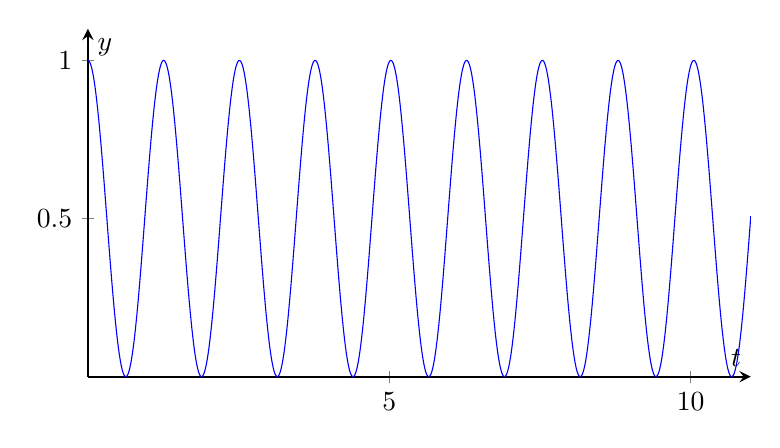
\begin{tikzpicture}
      \begin{axis}[
        axis lines=center,
        ymin=0,
        ymax=1.1,
        ylabel=$y$,
        xlabel=$t$,
        axis line style = thick,
        width=10cm,
        height=6cm,
        ytick={0, 0.5,1},
        xtick={0,5,10},
        ]
        \addplot[domain=0:11,samples=1000, blue]{(1+cos(deg(5*x)))/2};
      \end{axis}
    \end{tikzpicture}
  \end{center}
  \caption{(\ref{equ:polar})式の概形, $\omega_{1\perp}-\omega_{2\perp}=10$}
  \label{fig:polarplt}
\end{figure}

\begin{figure}[htbp]
  \begin{center}
    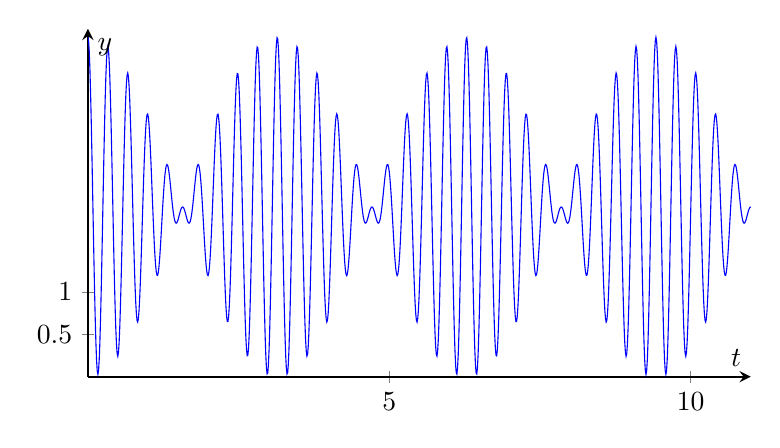
\begin{tikzpicture}
      \begin{axis}[
        axis lines=center,
        ymin=0,
        ymax=4.1,
        ylabel=$y$,
        xlabel=$t$,
        axis line style = thick,
        width=10cm,
        height=6cm,
        ytick={0, 0.5,1},
        xtick={0,5,10},
        ]
        \addplot[domain=0:11,samples=1000, blue]{2+2*(cos(deg(19*x)))*(cos(deg(x)))};
      \end{axis}
    \end{tikzpicture}
  \end{center}
  \caption{(\ref{equ:nopolar})式の概形, $a=10$, $b=9$}
  \label{fig:nopolarplt}
\end{figure}